% Chapter 5 -- structure from table of content.md; impersonal academic style

\reportchapter{5}{Evaluation and Conclusion}{Evaluation methodology, empirical results, interpretation, contributions, limitations, and future work.}

\section{Introduction}

This chapter reports how the platform defined in Chapters~2--4 was evaluated against a curated benchmark and how the results should be interpreted. The objective is not to claim definitive superiority over all political-analysis systems, but to measure end-to-end behavior of the deployed Graph-RAG stack: retrieval from ZVec and Neo4j, synthesis with citations, and optional reasoning modes. The presentation covers the evaluation methodology, metric families, quantitative results obtained on the live backend, limitations and threats to validity, contributions of the PFE, and directions for future work.

\section{Evaluation Methodology}

Evaluation was designed to test the system as a complete platform rather than as isolated components. The harness under \texttt{src/backend/evaluation} sends each benchmark question to the same HTTP query endpoint used by the React frontend, collects the generated answer together with retrieved chunks and graph facts, and scores the output against a reference answer. This protocol ensures that reported numbers reflect deployed behavior (ingestion state, indexes, reasoning mode, and judge configuration) rather than a mocked retrieval function.

\textbf{Dataset and question categories.} The primary benchmark is stored at \texttt{benchmark/questions.jsonl} and loaded by \texttt{dataset.py}. It contains \textbf{fourteen} questions grouped into four categories aligned with political intelligence use cases: \textbf{factual} (direct entity or event lookup), \textbf{relational} (connections between actors or institutions), \textbf{temporal} (chronology and dated events), and \textbf{comparative} (synthesis across several sources or positions). Each row includes a question, a reference answer (\texttt{ground\_truth}), optional source hints, and evidence document identifiers where applicable. The mix exercises both flat retrieval and graph-dependent reasoning described in Chapter~3.

\textbf{Evaluation pipeline.} Figure~\ref{fig:state-evaluation-pipeline} summarizes the flow. Each sample is submitted to the backend in one of three reasoning modes (\texttt{rag}, \texttt{cot}, or \texttt{reflexive}). The response supplies answer text, source previews, and graph facts; the metrics module then computes RAGAS-style scores via a Mistral judge. Errors and latency are logged per sample so that failed queries do not silently skew aggregates.

\begin{figure}[H]
    \centering
    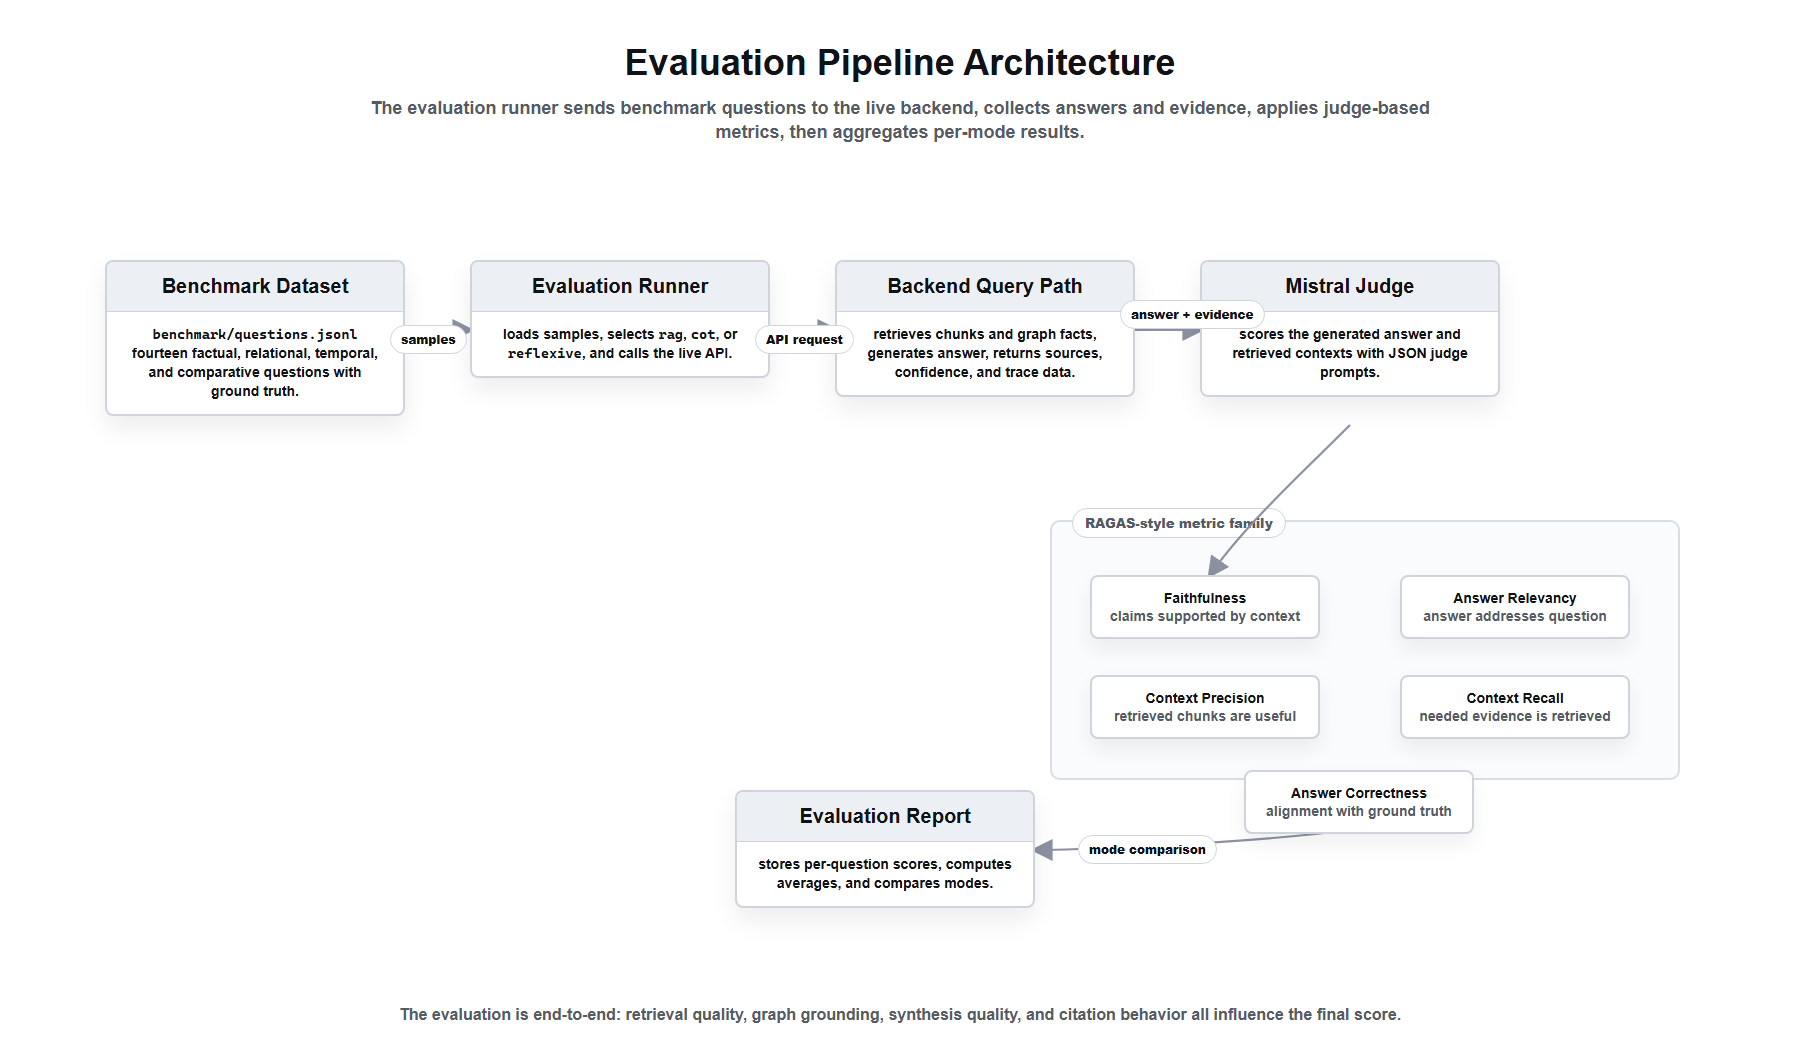
\includegraphics[width=0.96\textwidth,height=0.78\textheight,keepaspectratio]{images/state_evaluation_pipeline.png}
    \caption{Evaluation pipeline for querying the live backend and scoring generated answers.}
    \label{fig:state-evaluation-pipeline}
\end{figure}

\textbf{Experimental protocol.} The backend was invoked at \texttt{http://localhost:8001/api/v1/query} with \texttt{include\_sources=true} and \texttt{max\_hops=3}. Each of the fourteen benchmark questions was evaluated under \texttt{rag}, \texttt{cot}, and \texttt{reflexive} modes after MIPROv2 prompt optimization and corpus hardening. Each answer was judged on faithfulness, answer relevancy, context recall, and answer correctness (context precision is computed in the harness but omitted from the overview figure for readability). Aggregates are consolidated in \texttt{eval\_results.json} and per-mode files (\texttt{eval\_rag.json}, \texttt{eval\_cot.json}, \texttt{eval\_reflexive.json}); the reported run (May~2026) completed with zero backend errors on all samples.

\section{Evaluation Metrics and Results}

Three complementary metric families inform the analysis. Each answers a different quality question so that evaluation does not collapse into a single opaque score.

\textbf{Lexical metrics.} N-gram overlap compares the generated answer to the reference through contiguous word sequences, in the spirit of BLEU (precision-oriented) and ROUGE (recall-oriented) \cite{papineni-ngram,lin-rouge}. Lexical scores reward recovery of names, dates, institutions, and fixed expressions. They are strict: paraphrases that preserve meaning may score low. In political QA, lexical metrics are therefore used mainly to detect missing non-negotiable facts, not as the sole indicator of correctness.

\textbf{Semantic similarity.} Semantic Answer Similarity (SAS) measures whether two answers express the same meaning despite different surface wording \cite{risch-sas}. Embeddings and cosine similarity provide a softer signal than n-grams, which matters for relational and comparative questions where the system composes narrative answers from several evidence fragments. SAS complements lexical baselines when reference answers use alternate phrasing for the same geopolitical fact.

\textbf{RAGAS-style metrics.} The implemented harness follows the RAGAS philosophy: evaluate grounding and retrieval quality alongside the final answer \cite{ragas-paper,ragas-answer-correctness}. \textbf{Faithfulness} checks whether claims are supported by retrieved context. \textbf{Answer relevancy} measures alignment with the user question. \textbf{Context precision} and \textbf{context recall} assess whether retrieved passages contain useful and sufficient evidence. \textbf{Answer correctness} compares the generation to the ground truth through a Mistral judge (score in $[0,1]$ with short rationale). These metrics map directly to the validation criteria of Chapter~2 (grounded synthesis and inspectable evidence).

\textbf{Quantitative results.} Table~\ref{tab:mode-comparison} reports post-optimization mode-level means from \texttt{eval\_results.json} (fourteen questions, three modes, no request failures). In \texttt{rag} mode, answer correctness reaches \textbf{0.52} and answer relevancy \textbf{0.65}; faithfulness rises to \textbf{0.46} and context recall to \textbf{0.32} relative to the pre-optimization baseline. \texttt{cot} mode improves all four reported metrics (correctness \textbf{0.65}, relevancy \textbf{0.76}, faithfulness \textbf{0.58}, context recall \textbf{0.48}). \texttt{reflexive} mode achieves the strongest profile (correctness \textbf{0.80}, relevancy \textbf{0.92}, faithfulness \textbf{0.73}, context recall \textbf{0.64}), confirming that deeper reasoning and self-critique benefit political QA when retrieval supplies usable evidence.

\begin{table}[H]
\centering
\small
\setlength{\tabcolsep}{6pt}
\renewcommand{\arraystretch}{1.35}
\begin{tabularx}{\textwidth}{@{}>{\bfseries\raggedright\arraybackslash}p{2.2cm}>{\centering\arraybackslash}X>{\centering\arraybackslash}X>{\centering\arraybackslash}X>{\centering\arraybackslash}X@{}}
\toprule
\rowcolor{lightblue}
Mode & Correct. & Relev. & Faithful. & Ctx.\ recall \\
\midrule
RAG & 0.52 & 0.65 & 0.46 & 0.32 \\
CoT & 0.65 & 0.76 & 0.58 & 0.48 \\
Reflexive & 0.80 & 0.92 & 0.73 & 0.64 \\
\bottomrule
\end{tabularx}
\caption{Post-optimization RAGAS-style scores by reasoning mode (14-question benchmark, May 2026).}
\label{tab:mode-comparison}
\end{table}

Figure~\ref{fig:evaluation-results-overview} visualizes the same mode-level comparison. The monotonic gain from RAG to CoT to reflexive mode indicates that prompt optimization and reasoning depth compound; context recall remains the metric with the largest absolute lift under reflexive mode, while still leaving room for retrieval hardening.

\begin{figure}[H]
    \centering
    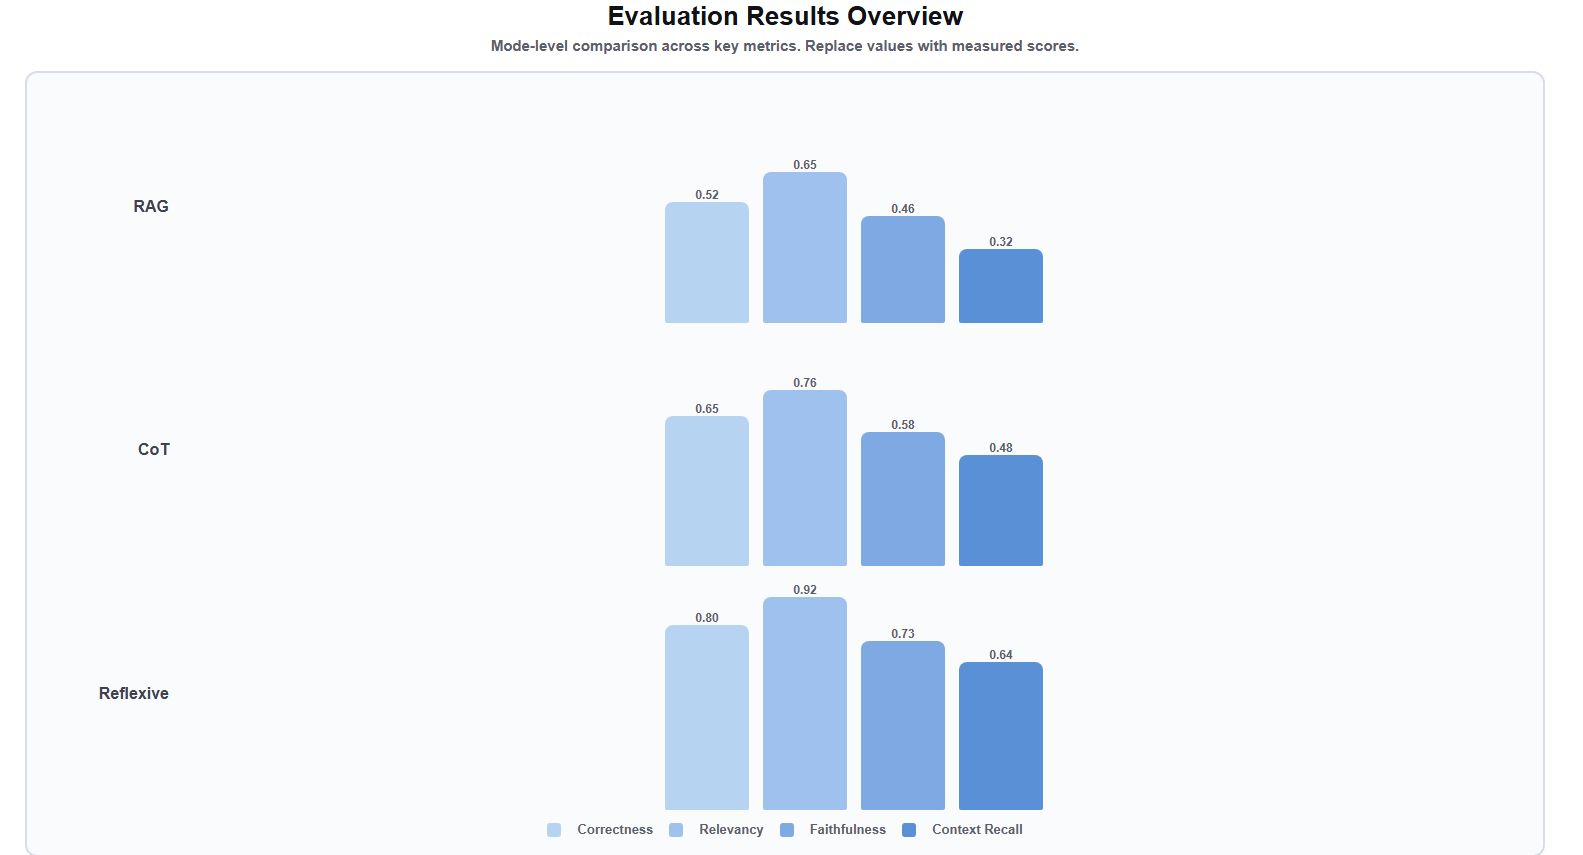
\includegraphics[width=0.92\textwidth,keepaspectratio]{images/evaluation_results_overview.png}
    \caption{Post-optimization overview of mean RAGAS-style scores by reasoning mode (correctness, relevancy, faithfulness, context recall).}
    \label{fig:evaluation-results-overview}
\end{figure}

\section{Interpretation and Limitations}

\textbf{Performance analysis.} Post-optimization scores show that the platform understands questions and grounds answers more reliably than in the first evaluation pass. \texttt{rag} mode already reaches moderate correctness and relevancy; \texttt{reflexive} mode nearly doubles context recall relative to \texttt{rag} (\textbf{0.64} vs.\ \textbf{0.32}), which supports the design choice of offering selectable reasoning depth in the UI. Remaining gaps appear on niche factual items where the corpus still lacks the exact entity or event named in the ground truth, even when the model abstains safely rather than hallucinating.

\textbf{Retrieval bottlenecks.} Context recall improves with mode complexity but remains the lowest absolute metric in \texttt{rag} mode (\textbf{0.32}). Contributing factors include corpus gaps, chunk-boundary effects, syndicated or noisy articles passing quality gates, and insufficient graph-aware reranking on the first retrieval hop. Further gains should come from ingestion expansion and reranking before additional reasoning hops, in line with validation criteria in Chapter~2.

\textbf{Threats to validity.} Four limitations bound the conclusions. \emph{Corpus coverage:} scores depend on what was ingested at evaluation time. \emph{Judge bias:} LLM-based scoring may favor fluent answers or penalize careful abstention. \emph{Temporal drift:} political facts change; the fourteen-question snapshot does not guarantee stable scores after new ingestion. \emph{Benchmark size:} the set is representative but small; enlarged benchmarks and human analyst ratings would strengthen external validity.

\section{Contributions}

The PFE delivers contributions at methodological, technical, and operational levels.

\textbf{Methodological.} A project-specific evaluation protocol combines lexical and semantic families from the literature with RAGAS-style grounding metrics executed on the live API. Question categories (factual, relational, temporal, comparative) tie metrics to analyst workflows rather than to generic QA benchmarks alone.

\textbf{Technical.} An end-to-end Graph-RAG platform integrates autonomous ingestion, ZVec semantic retrieval, Neo4j traversal, selectable reasoning modes, DuckDuckGo-augmented live search, a React analytical workspace, and containerized observability---addressing the integration gap identified in Chapter~1.

\textbf{Operational.} Staged ingestion scripts, database diagnostics, MIPROv2 prompt optimization, and the evaluation harness (\texttt{runner.py}, \texttt{compare\_modes.py}) make ingestion, retrieval, and scoring reproducible for iterative engineering.

\section{Future Work}

\textbf{Retrieval improvements.} Graph-aware reranking, stricter source filtering, query expansion, and temporal filters on edges should raise context precision and recall. Re-embedding and chunking experiments on the MongoDB corpus are the highest-impact lever given current metrics.

\textbf{Evaluation expansion.} The same fourteen-question protocol should be extended to a larger benchmark with lexical and SAS columns reported alongside RAGAS metrics, and with human analyst ratings on a stratified subset to cross-check the Mistral judge.

\textbf{Temporal modeling extensions.} Stronger validity intervals on relations, time-scoped graph queries at retrieval time, and alignment between structured legislative dates and graph edges would address weak temporal correctness scores.

\section{Conclusion}

The platform demonstrates that political Graph-RAG can be engineered as a sovereign, inspectable pipeline from ingestion to cited answers. Post-optimization evaluation on fourteen curated questions shows measurable gains across reasoning modes, with reflexive mode reaching strong relevancy and correctness while context recall remains the main lever for further improvement. The work contributes a reproducible architecture, an evaluation harness tied to production APIs, and evidence that prompt optimization and reasoning depth matter as much as raw retrieval. The bridge between unstructured political information and structured, grounded reasoning remains open for incremental hardening rather than closed as a finished product.
